\documentclass{beamer}
\usetheme{CambridgeUS}

% Title page details:
\title{GoTalk}
\author{Swasti \and Shreya \and Krishika \and Samriddhi}
\date{\today}

\begin{document}

% Title frame
\begin{frame}
    \titlepage
    \centering HACKTIVISTS
\end{frame}

% Idea frame
\begin{frame}{PROJECT AIM}
    To develop a real-time chat web application with bidirectional communication and chat history retrieval using Go, WebSocket and Firebase majorly.   
    \\
    Our main aim is to Learn the Go language and Firebase and learn how to establish a client-server connection using WebSocket .
\end{frame}

\section{Tech Stack}
\begin{frame}{Tech Stack}
    \begin{itemize}
        \item \textbf{Frontend}
        \begin{itemize}
            \item HTML/CSS
            \item JavaScript
            \item Bootstrap/Tailwind CSS
        \end{itemize}
        \item \textbf{Backend}
        \begin{itemize}
            \item Go (Golang)
            \item Gorilla WebSocket
            \item Firebase Realtime Database
        \end{itemize}
    \end{itemize}
\end{frame}

% Aim frame
\begin{frame}{COMPLETED TASKS}
    \begin{itemize}
        \item Established bidirectional communication using WebSocket.
        \item Implemented past chat retrieval feature.
        \item Integrated Firebase Console for real-time Database management.
        \item Successfully stored all messages in the firebase real-time database.
        \item Added basic styles to the user interface. 
   \end{itemize}
\end{frame}

\begin{frame}{CURRENT STATUS}
    \begin{minipage}[t]{0.3\textwidth}
        \centering
        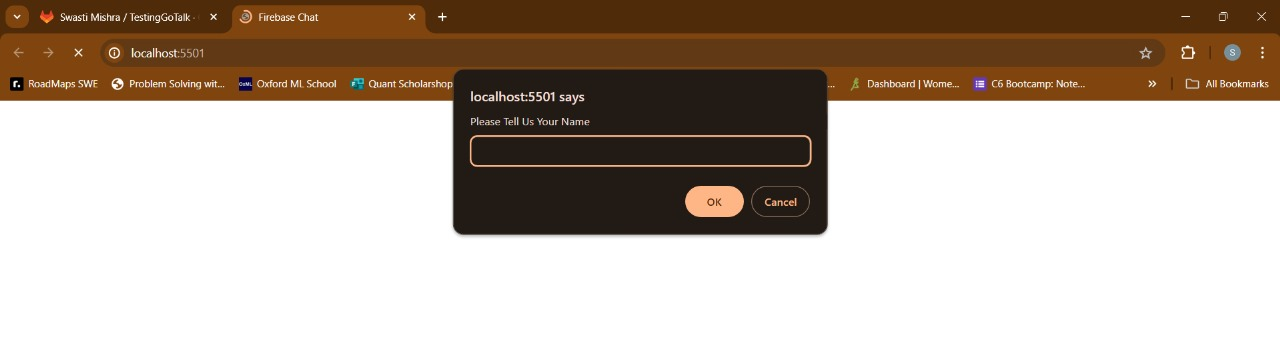
\includegraphics[width=\textwidth]{openpage.jpg}
    \end{minipage}
    \hfill
    \begin{minipage}[t]{0.3\textwidth}
        \centering
        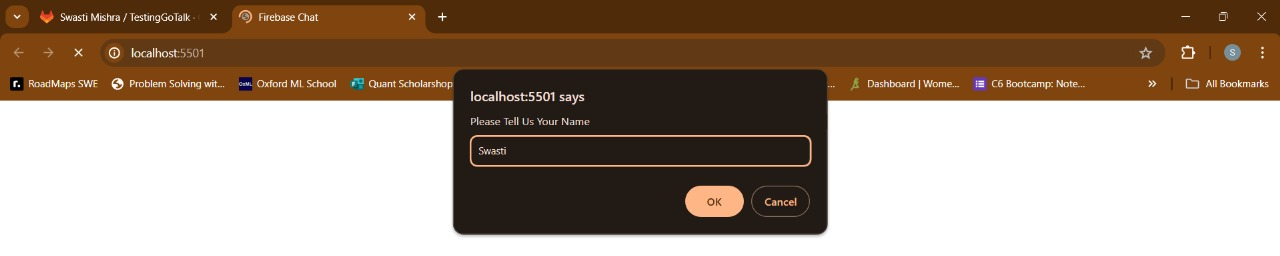
\includegraphics[width=\textwidth]{entername}
    \end{minipage}
    \hfill
    \begin{minipage}[t]{0.3\textwidth}
        \centering
        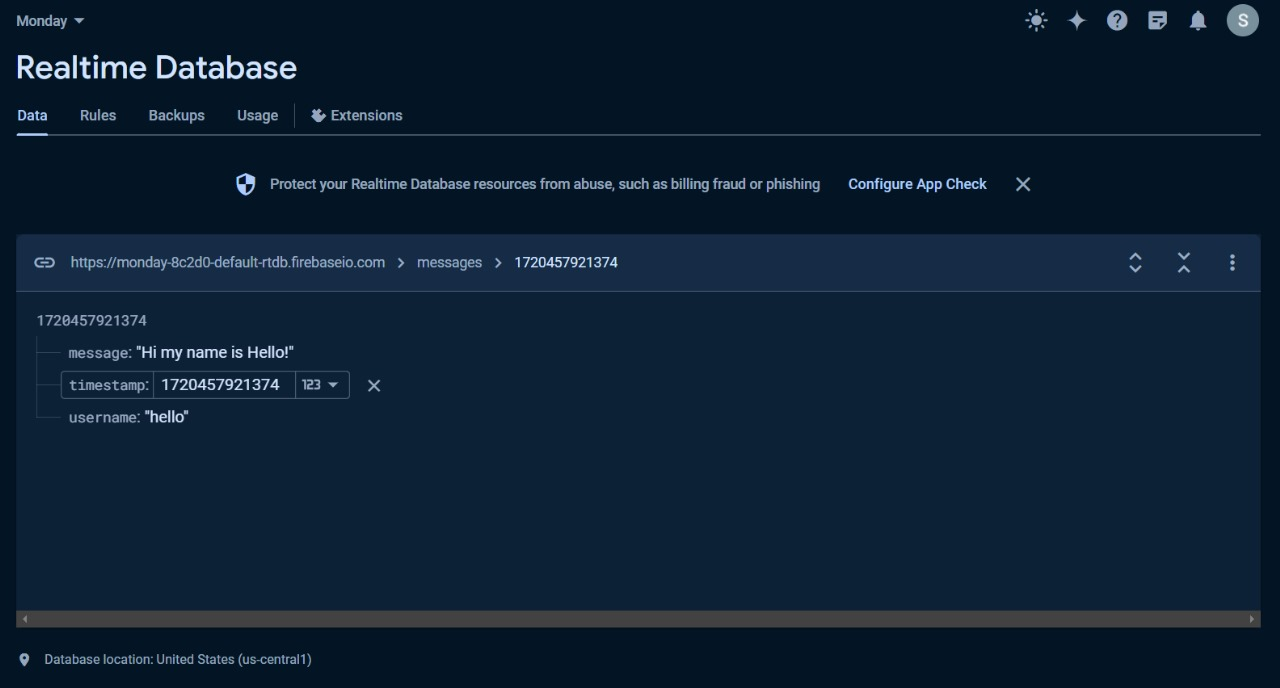
\includegraphics[width=\textwidth]{database.jpg}
    \end{minipage}

    \vspace{0.5cm}

    \begin{minipage}[t]{0.3\textwidth}
        \centering
        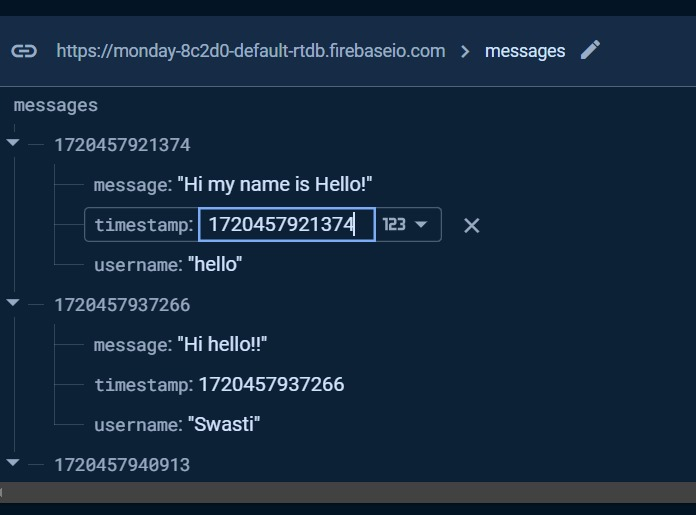
\includegraphics[width=\textwidth]{firebase.jpg}
    \end{minipage}
    \hfill
    \begin{minipage}[t]{0.3\textwidth}
        \centering
        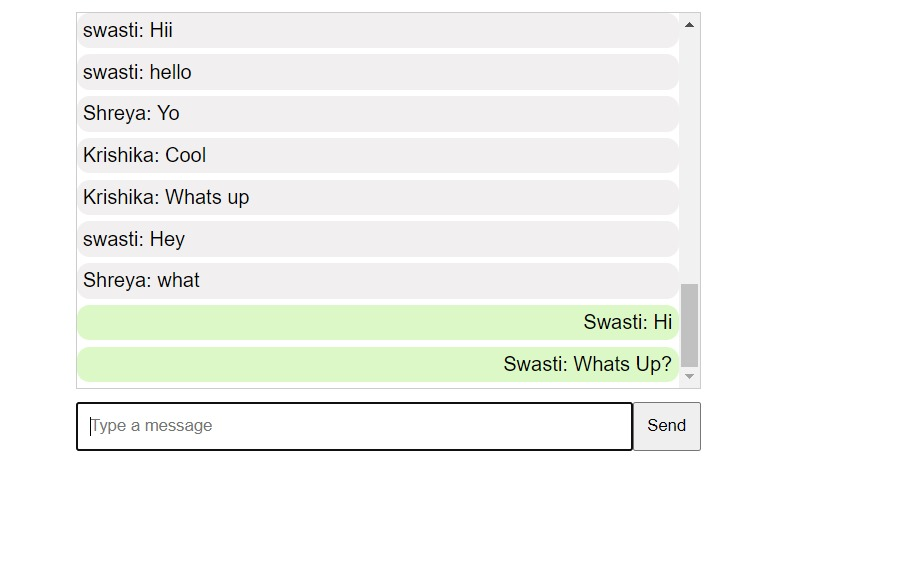
\includegraphics[width=\textwidth]{chatinterface.jpg}
    \end{minipage}
    \hfill
    \begin{minipage}[t]{0.3\textwidth}
        \centering
        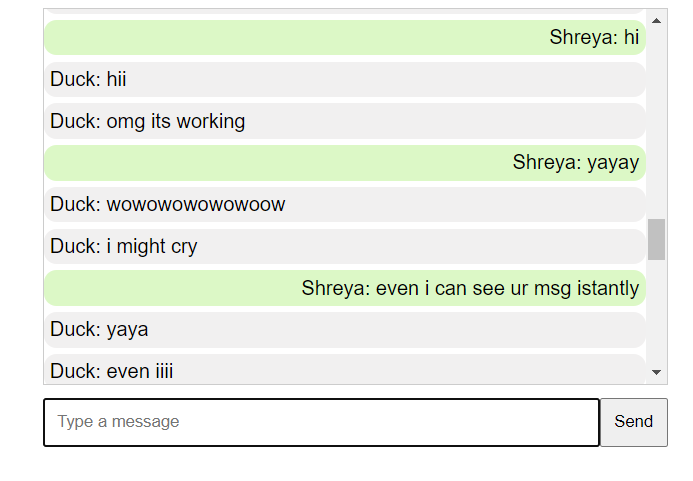
\includegraphics[width=\textwidth]{interface.png}
    \end{minipage}
\end{frame}


\begin{frame}{ISSUES WE ARE FACING}
    \begin{itemize}
        \item On reloading the user is directed to re-enter the name in the pop-up shown. \\
        on re-entering the name the past messages stay the same but this gives user a chance to change their name frequently which might be annoying and this is not what we intended for.
        
        \item so we are working on changing this so that the program remembers that the user is the same who logged in previously.
    \end{itemize}
\end{frame}

\begin{frame}{CHALLENGES WE FACED}
    \begin{block}{Problems Faced :}
        \begin{itemize}
            \item Initial issues with WebSocket integration.
            \item UI/UX design not fully polished. 
        \end{itemize}
    \end{block}
    
    \begin{block}{Mitigation Strategies: }
        \begin{itemize}
            \item Collaborated to troubleshoot WebSocket issues.
            \item planning to refine UI/UX in the next phase.
        \end{itemize}
    \end{block}
\end{frame}

\begin{frame}{WORK IN PROGRESS}
    \begin{itemize}
        \item Improving UI/UX
        \item User authentication.
        \item Testing and debugging the application
        \\
        Main task : to make sure that the program remembers the user when run again.
    \end{itemize}
\end{frame}

\section{Timeline}
\begin{frame}{Timeline}
    \begin{block}{Week 1 - 1/08/2024 - 7/08/2024}
        \begin{itemize}
            \item Installation
            \item Basic HTTP server
            \item WebSocket integration
            \item User Authentication using Firebase
        \end{itemize}
    \end{block}
    
    \begin{block}{Week 2 : 8/07/24 - 14/07/24}
        \begin{itemize}
            \item Handling messages
            \item Chat history 
            \item User interface
            \item Documentation
        \end{itemize}
    \end{block}
\end{frame}

% Procedure frame
\begin{frame}{UPCOMING TASKS}
    \begin{itemize}
        \item Refining and enhancing the user interface.
        \item Conducting extensive testing and fixing any bugs
        \item Gathering user feedback for further improvements.
        \item Ensure smooth and reliable chat experience. 
    \end{itemize}
\end{frame}

\begin{frame}{CONCLUSION}
    \begin{itemize}
        \item Successfully established bidirectional communication and chat history retrieval using WebSocket and Firebase
        \item Basic UI Implemented, with further improvements planned.
        \item Working on user interface.
    \end{itemize}
\end{frame}

% Thank You frame
\begin{frame}{Thank You}
    \centering
    \Huge Thank You!
\end{frame}

\end{document}
